\newpage
\chapter{Transformation Zeitreihe zu Netzwerk}
Ziel unseres Forschungsprojektes ist es unter anderem verschiedene Algorithmen, zur Ausrei�er Erkennung in Netzwerken, auf Zeitreihendaten anzuwenden. Als erstes m�ssen hierzu die Zeitreihen in ein Netzwerk umgewandelt werden, dieser Schritt wird in diesem Kapitel erl�utert. Je nach Ausrei�er-Erkennung Algorithmus, muss die Transformation leicht unterschiedlich durchgef�hrt werden. Aus diesem Grund wird in \autoref{chap:trsnsNeti}, \autoref{chap:trsnsMidas} und \autoref{chap:trsnsMidasR} erl�utert wie die Umwandlung f�r die jeweiligen Algorithmen funktioniert.
\section{Netsimile}
\label{chap:trsnsNeti}
Der erste Schritt der Transformation ist, die Zeitreihe in kleinere Intervalle aufzusplitten. Anschlie�end kann f�r jedes der Intervalle ein Netzwerk berechnet werden. Die L�nge des Intervalls kann als Hyperparameter an den Algorithmus �bergeben werden. Je nach Zeitreihe funktionieren unterschiedliche Intervallgr��en besser oder schlechter. Insofern die Zeitreihe eine Saisonalit�t aufweist, kann diese bestimmt und als Intervallgr��e genutzt werden.
\workTodo{�berpr�fen ob Saisonalit�t der richtige Begriff ist.}\\
Um die einzelne Zeitintervalle in ein Netzwerk umzuwandeln, wird zun�chst die Distanz zwischen den einzelnen Elementen des Zeitintervalls berechnet. Hierzu wird auf das in \citep[vgl.][S.~2-3]{10.3389/fphy.2019.00194} vorgestellte Distanzma� zur�ckgegriffen. Insofern f�r p = 2 eingesetzt wird, handelt es sich um die euklidische Distanz. Die Abst�nde bilden die Kantengewichte zwischen den jeweiligen Elementen im Netzwerk. Die Elemente der Zeitreihe bilden die Knoten des Netzwerks. Die Netzwerke werden intern als Adjazenzmatrizen gespeichert.
$$D_{ij}=\left(\sum_{k} \left|v_{k}^{i}-v_{k}^{j}\right|^{p}\right)^{1/p}$$
 Im n�chsten Schritt m�ssen die Netzwerke in CSV-Dateien gespeichert werden, sodass der  Netsimile Algorithmus die Daten einlesen kann. Dazu wird f�r jede Kante des Netzwerks eine  Zeile im der Datei, mit folgendem Format generiert: Ursprungsknoten, Zielknoten, Gewichtung. F�r jedes Zeitintervall muss eine einzelne CSV-Datei angelegt werden. Der Netsimile Algorithmus vergleicht...

\begin{figure}[H]
	\centering
	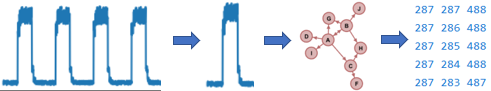
\includegraphics[width=13cm]{fig/tsToNet/tsToCsv}
	\caption{Umwandlung einer Zeitreihe in Netzwerk}
	\label{img:tsToNet}
\end{figure}
\workTodo{Das Netzwerk aus der Grafik noch ab�ndern}



\section{MIDAS}
\label{chap:trsnsMidas}
Die Transformation der Zeitreihe in mehrere Netzwerke funktioniert f�r den MIDAS Algorithmus gleich wie in \autoref{chap:trsnsNeti}. Allerdings kann der Algorithmus teilweise bessere Ergebnisse erzielen, wenn f�r p eine Zahl gr��er als zwei eingesetzt wird. Dadurch werden gr��ere Abst�nde zwischen Elementen st�rker gewichtet.\\
Au�erdem erwartet der MIDAS Algorithmus f�r die Netzwerkdaten ein anderes �bergabeformat. Hierbei k�nnen alle Daten der jeweiligen Zeitabschnitte in einen CSV-File geschrieben werden. Die CSV-Datei muss dabei folgenderma�en strukturiert sein: Ursprungsknoten, Zielknoten, Zeitintervall. Es ist nicht m�glich die Kantengewichtung direkt an den Algorithmus zu �bergeben. Um die Kantengewichtung trotzdem �bergeben zu k�nnen, wird die gleiche Kante mehrmals in Abh�ngigkeit der Gewichtung an den Algorithmus �bergeben.
Wie funkt Midas ganz kurz..


\begin{figure}[H]
	\centering
	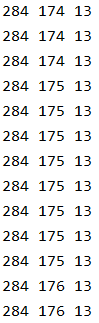
\includegraphics[width=2cm]{fig/tsToNet/midasData}
	\caption{Datensatz Midas}
	\label{img:tsToNetMiData}
\end{figure}
\workTodo{Vielleicht kleineren Auszug aus Datensatz verwenden}


\section{MIDAS-R}
\label{chap:trsnsMidasR}
\workTodo{Hab hier das mit der Hauptkomponentenzerlegung gemacht. Wenn es Ergebnisse hierf�r gibt. Kann ich das hier noch erkl�ren}
